   \begin{figure}[]
        \centering
		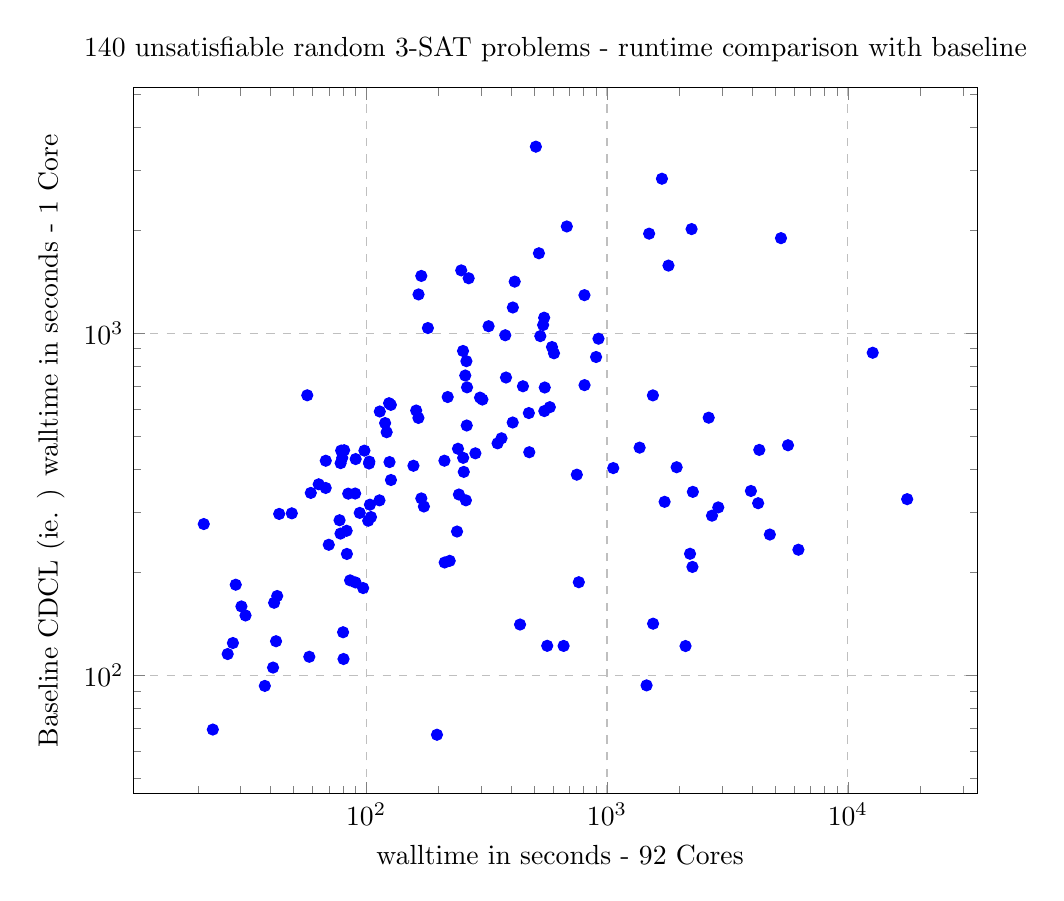
\begin{tikzpicture}
		\begin{axis}[
			title={140 unsatisfiable random 3-SAT problems - runtime comparison with baseline},
			xlabel={\dagster\ walltime in seconds - 92 Cores},
			ylabel={Baseline CDCL (ie. \tinisat) walltime in seconds - 1 Core},
			%xmin=0, xmax=0.25,
			%ymin=10.00, ymax=100000.00,
			ymode=log,
			xmode=log,
			%xtick={0,0.05,0.1,0.15,0.2,0.25},
			%ytick={0,20,40,60,80,100},
			%yticklabel=$\pgfmathprintnumber{\tick}\%$,
			legend pos=south east,
			ymajorgrids=true,
			xmajorgrids=true,
			grid style=dashed,
			xticklabel style={/pgf/number format/fixed},
			width = 350,
			height = 300
		]


\addplot[color=blue,only marks] coordinates {
(42.26,125.745)(119.867,545.704)(2728.217,292.677)(67.931,352.727)(21.179,276.65)(322.382,1047.232)(240.595,459.067)(78.358,416.759)(660.406,121.842)(1550.594,657.514)(43.543,296.155)(261.625,536.902)(80.2,133.574)(506.602,3505.237)(121.648,513.245)(1061.421,403.139)(97.171,179.823)(41.486,162.886)(126.765,372.093)(806,1290.684)(4240.705,318.299)(2643.525,565.834)(590.973,910.356)(351.253,476.16)(84.247,339.432)(447.676,699.161)(763.726,187.065)(113.936,589.902)(77.559,283.815)(180.447,1034.351)(1690.419,2824.716)(49.133,297.309)(27.976,124.23)(1553.507,141.486)(101.967,282.867)(1495.695,1952.363)(104.73,289.984)(2896.473,309.438)(406.422,1187.694)(126.619,616.863)(102.826,415.73)(266.463,1446.01)(549.248,591.68)(211.846,213.583)(23.089,69.41)(124.491,623.812)(90.453,428.356)(248.186,1524.726)(921.673,962.741)(26.615,115.363)(173.687,311.332)(1459.816,93.42)(1799.701,1574.52)(521.555,1711.07)(80.547,111.57)(254.275,393.006)(564.572,121.919)(196.821,67.018)(475.597,448.536)(169.425,1468.822)(380.813,741.443)(1365.755,462.605)(30.35,158.917)(2244.52,2013.101)(364.733,492.594)(2262.841,207.311)(1734.328,321.255)(435.473,140.696)(81.024,454.584)(79.552,431.68)(548.294,1108.946)(378.084,985.383)(602.305,872.929)(222.258,215.967)(37.967,93.092)(4742.795,257.769)(262.324,694.06)(58.079,113.235)(6232.027,232.727)(242.733,337.452)(1946.22,405.46)(260.738,827.722)(169.469,328.716)(113.582,324.442)(749.381,385.727)(164.833,564.966)(5641.305,470.067)(528.534,979.646)(78.755,453.489)(103.65,315.154)(28.745,183.927)(2118.508,121.737)(161.348,593.823)(58.911,341.096)(63.529,361.476)(3958.052,345.572)(82.985,264.38)(542.899,1055.738)(257.885,751.644)(90.344,186.763)(2271.456,343.524)(157.159,409.5)(42.722,170.464)(252.424,886.519)(98.35,453.322)(165.033,1296.811)(297.089,647.719)(78.255,259.416)(56.956,657.919)(303.857,639.407)(2211.474,226.46)(551.438,693.299)(5275.306,1894.192)(218.042,650.364)(413.741,1413.715)(41.065,105.315)(259.474,324.486)(238.411,263.036)(405.909,547.863)(900.781,851.23)(125.022,419.773)(67.987,423.571)(806.681,704.496)(680.987,2048.929)(90.016,339.74)(94.047,298.174)(12679.367,875.948)(83.19,226.217)(4287.566,455.582)(85.779,189.365)(103.114,420.958)(252.831,431.952)(17628.641,327.106)(31.568,149.551)(69.96,240.616)(284.138,445.204)(578.942,607.365)(473.695,583.777)(211.334,423.656)
}node[pos=0.8](endofplotsquare){} ;


		\end{axis}
		\end{tikzpicture}
		%\vspace{-18pt}
  \caption[Scatterplot of Tinisat against Dagster for random unsatisfiable 3Sat instances]{Logscale scatter plot of runtime distributions of \tinisat\ (vertical) and \dagster\ using 92 cores (horizontal) on pseudo-random unsatisfiable $3$-Satisfiability problem instances.\label{fig:3UNSAT_140random}}
    \end{figure}
